\subsection*{Problema 01}

\textbf{Enunciado:} Evaluar la integral definida mediante sumas de Riemann usando una partición regular:
\begin{align*}
\int_{-3}^{1} x \, dx
\end{align*}

\textbf{Solución:} Para evaluar la integral definida mediante la definición de límite de una suma de Riemann, consideramos una partición regular del intervalo $[-3, 1]$ en $n$ subintervalos de igual longitud $\Delta x$.

La longitud del intervalo es $\Delta x$:
\begin{align*}
\Delta x &= \dfrac{1 - (-3)}{n} = \dfrac{4}{n}
\end{align*}

Los extremos derechos de cada subintervalo, denotados como $x_i$, se definen mediante la fórmula:
\begin{align*}
x_i &= a + i\Delta x \\
x_i &= -3 + i\left(\dfrac{4}{n}\right)
\end{align*}

Evaluamos la función $f(x) = x$ en cada punto $x_i$:
\begin{align*}
f(x_i) &= -3 + \dfrac{4i}{n}
\end{align*}

Planteamos la suma de Riemann usando el extremo derecho:
\begin{align*}
S_n &= \sum_{i=1}^{n} f(x_i) \Delta x \\
S_n &= \sum_{i=1}^{n} \left( -3 + \dfrac{4i}{n} \right) \dfrac{4}{n}
\end{align*}

Distribuimos y aplicamos las propiedades de linealidad de la suma:
\begin{align*}
S_n &= \dfrac{4}{n} \left[ \sum_{i=1}^{n} (-3) + \dfrac{4}{n} \sum_{i=1}^{n} i \right] \\
S_n &= \dfrac{4}{n} \left[ -3n + \dfrac{4}{n} \cdot \dfrac{n(n+1)}{2} \right]
\end{align*}

Simplificamos el segundo término dentro del corchete:
\begin{align*}
S_n &= \dfrac{4}{n} \left[ -3n + \dfrac{2n(n+1)}{n} \right] \\
S_n &= \dfrac{4}{n} [ -3n + 2(n+1) ] \\
S_n &= \dfrac{4}{n} [ -3n + 2n + 2 ] \\
S_n &= \dfrac{4}{n} ( -n + 2 )
\end{align*}

Multiplicamos por $\dfrac{4}{n}$:
\begin{align*}
S_n &= -\dfrac{4n}{n} + \dfrac{8}{n} \\
S_n &= -4 + \dfrac{8}{n}
\end{align*}

Calculamos el límite cuando $n \to \infty$ para hallar el valor exacto de la integral definida:
\begin{align*}
\int_{-3}^{1} x \, dx &= \lim_{n \to \infty} S_n \\
&= \lim_{n \to \infty} \left( -4 + \dfrac{8}{n} \right) \\
&= -4 + 0 = -4
\end{align*}

El valor de la integral definida es $-4$.

\begin{figure}[H]
	\centering
	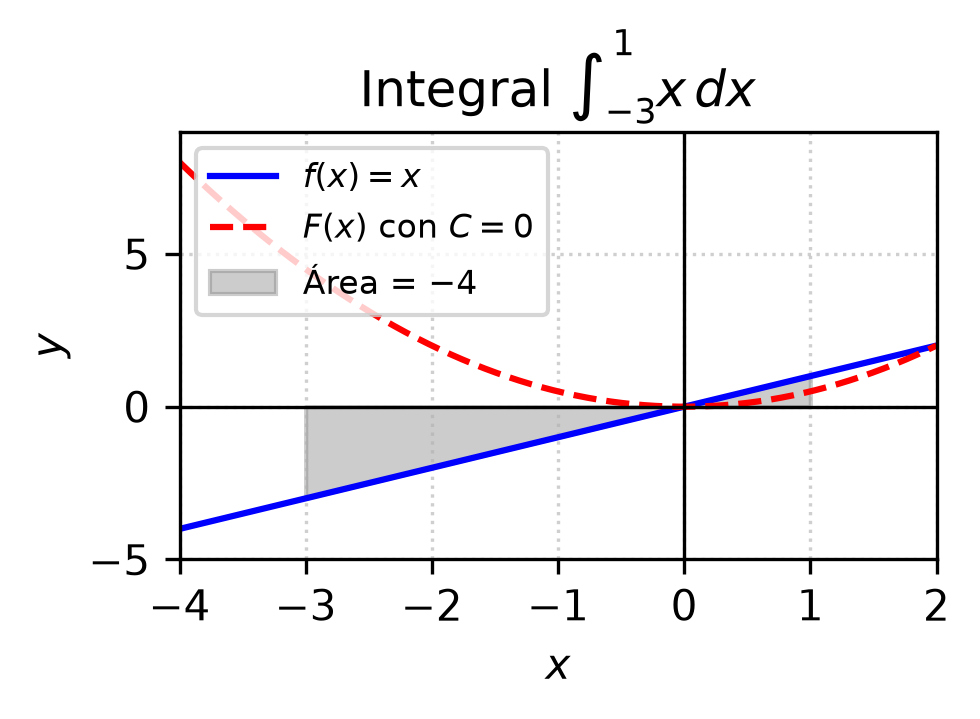
\includegraphics[width=\columnwidth]{semana_06/graficas/SEM06_P01_grafica.png}
	\caption{Representación gráfica de $f(x)$ y su antiderivada $F(x)$ evaluada para la constante de integración $C = 0$ (Problema 01).}
	\label{fig:problema01}
\end{figure}
